\documentclass[a4paper,11pt,oneside,titlepage,openany,onecolumn]{scrreprt}

%%%%%%%%%%%%%%%%%%%%%%%%%%%%%%%%%%%%%%%%%%%%%%%%%%%%%%%%%%%%%%%%%%%%%%%%%%%%%%%%%%%%%%

% General settings (input encoding, font encoding, font, language)
% ****************************************************************************************
\usepackage[utf8]{inputenc} % character encoding used in input file
\usepackage[T1]{fontenc} % specifies the encoding used in the fonts
\usepackage{lmodern} % provides more support for non-ASCII characters than cm-super
\usepackage{microtype} % improves line-filling when using PDFLaTeX
\usepackage[ngerman,english]{babel} % last language is considered the main one
%\usepackage{helvet}
\renewcommand{\familydefault}{\sfdefault} % select a sans serif font family
%
% ****************************************************************************************

% ****************************************************************************************
% Basic packages (graphics, tables, code highlighting, epigraphs)
% ****************************************************************************************
\usepackage{graphicx} % provides enhanced support for including graphics and images
% \usepackage{epstopdf}
\graphicspath{{img/}} % list of directories in which to search for graphics files 
\usepackage[table]{xcolor} % extends the color capabilities of LaTeX
\usepackage{color}
\definecolor{MSBlue}{rgb}{.204,.353,.541} 
\definecolor{trueblue}{rgb}{0.0, 0.45, 0.81}
\definecolor{onyx}{rgb}{0.06, 0.06, 0.06}
\definecolor{mygruen}{rgb}{0.4660, 0.6740, 0.1880}
\definecolor{plotblue}{rgb}{0, 0.4470, 0.7410}
\definecolor{myrot}{rgb}{0.8500, 0.3250, 0.0980}
\definecolor{mygreen}{RGB}{28,172,0} % Matlab comment
\definecolor{mylilas}{RGB}{170,55,241} % Matlab String
\definecolor{MCIBLUE}{RGB}{0,73,131}
\usepackage{tabularx} % extends functionality of the traditional tabular environment
\usepackage{array}
\usepackage{booktabs}
\usepackage{dcolumn}
\usepackage{multirow}

\usepackage{grffile} % improves support for file names with multiple dots
\usepackage{minted} % used to format and highlight programming language source code
% \usepackage{tocloft} % provides means of controlling the typographic design of the ToC
\KOMAoptions{toc=flat} % Glatte Abstände
\KOMAoptions{toc=indent} % Eingerückte Ebenen im Inhaltsverzeichnis
\setlength{\marginparwidth}{2cm}
\usepackage{todonotes}
\usepackage{pst-all} %% erweiterte Zeichenbefehle

% ****************************************************************************************
% Drawing and plotting
% ****************************************************************************************
\usepackage{pgfplots} % provides a high-level interface for creating plots and charts
\pgfplotsset{compat=newest} % sets the compatibility level to the newest version
\usetikzlibrary{plotmarks} % provides various markers (symbols) that can be used
\usetikzlibrary{arrows.meta} % allows customization of arrow tips for paths and arrows
\usepgfplotslibrary{patchplots} % provides additional functionality for handling patches
\usepgfplotslibrary{external} % provides functionality for externalizing plots
\tikzexternalize % activates the externalization feature for TikZ
\newlength\figureheight % declares a new length used to store used to store dimensions
\newlength\figurewidth % declares a new length used to store used to store dimensions
\usepackage{circuitikz} % used for drawing electrical circuits
\usepackage{tikz}
\usepackage{tikzscale}

% ****************************************************************************************
% Mathematics and physics
% ****************************************************************************************
\usepackage{amsmath,amssymb,amsfonts,amstext}
\usepackage{mathtools}
\usepackage{mathrsfs}

%% -> SI-Einheiten
\usepackage{siunitx}
% Einstellungen für SI-Einheiten
\sisetup{
	locale = DE,                        % Deutsche Einstellungen
	output-decimal-marker = {,},        % Dezimaltrennzeichen auf "," setzen
	exponent-product = \cdot,           % Exponenten mit "·" trennen
	per-mode = symbol-or-fraction,      % "pro" als Symbol oder Potenz
	parse-numbers = true,               % Automatische Nummerninterpretation
	bracket-numbers = false             % Entfernt Klammern bei negativen Exponenten
}

% ****************************************************************************************
% Referencing and citing
% ****************************************************************************************
\usepackage[
	format=plain,% typeset caption as normal paragraph
	labelformat=simple,% typeset label as name and number
	labelsep=period,% caption label and text separated by period and space
	textformat=simple,% caption text typeset as is (without additional formatting)
	justification=justified,% sets the justification of the caption text to be justified
	singlelinecheck=true,% automatically center short captions
	font=small,% set font size to small
	labelfont=bf,% set bold font for label
	width=.75\textwidth% set fixed width for caption
]{caption} % customize the formatting of captions
\usepackage{subcaption}
\captionsetup[figure]{
	labelfont=bf,                   % Beschriftung für Abbildungen fett
	textfont=normal,                % Text normal
	labelsep=space,                 % Punkt nach der Beschriftung
	%belowskip=10pt
}
\captionsetup[table]{
	labelfont=bf,                   % Beschriftung für Tabellen fett
	textfont=normal,                % Text normal
	labelsep=space,                 % Punkt nach der Beschriftung
	belowskip=10pt
}
% Titel von Abbildungen und Tabellen ändern
\renewcommand\figurename{Abbildung}
\renewcommand\tablename{Tabelle}
% ****************************************************************************************

% \usepackage{hyperref} % hypertext marks (should be loaded last but before geometry)
% \hypersetup{
%     colorlinks,% colours the text of links and anchors (instead of borders)
% 	linkcolor={MCIBLUE},%
% 	citecolor={MCIBLUE},%
% 	urlcolor={MCIBLUE},%
%   % pdftitle={\thesisTitle},% PDF display and information options
% 	% pdfsubject={\thesisType},%
% 	% pdfauthor={\thesisStudent},%
% 	pdfkeywords={thesis},%
% 	pdfcreator={pdflatex},%
% 	pdfproducer={LaTeX with hyperref}%
% }
\usepackage[
bookmarks=true,
bookmarksopen=true,
bookmarksnumbered=true,
pdfborder={0 0 0},
colorlinks=true,
linkcolor=MCIBLUE,
citecolor=MCIBLUE,
urlcolor=MCIBLUE
]{hyperref}
\usepackage[capitalise]{cleveref} % enhances cross-referencing features
\crefformat{equation}{(#2#1#3)}
\Crefformat{equation}{Equation~(#2#1#3)}
\crefname{figure}{Abbildung}{Abbildungen} % Singular und Plural für Abbildungen
\crefname{table}{Tabelle}{Tabellen}       % Singular und Plural für Tabellen
\crefname{equation}{Gleichung}{Gleichungen} % Singular und Plural für Gleichungen

% \Crefname{figure}{Abbildung}{Abbildungen} % Für den Satzbeginn mit großem Anfangsbuchstaben
% \Crefname{table}{Tabelle}{Tabellen}
% \Crefname{equation}{Gleichung}{Gleichungen}
% ****************************************************************************************

% ****************************************************************************************
% Bibliography settings
% ****************************************************************************************
% IEEEtran BibTeX style downloaded from: https://www.ctan.org/pkg/ieeetran
\bibliographystyle{IEEEtran} % choose the reference style
%
% ****************************************************************************************
% Glossary (acronyms, list of symbols) settings
% ****************************************************************************************
\usepackage[acronym,nomain,nonumberlist,nopostdot,sort=def,toc]{glossaries}
\renewcommand*{\glstextformat}[1]{\textcolor{black}{#1}} % make links appear black
\newglossary[slg]{symbolslist}{syi}{syg}{List of Symbols} % define custom glossary
\glsaddkey% define custom key
	{unit}% key
	{\glsentrytext{\glslabel}}% default value
	{\glsentryunit}% command analogous to \glsentrytext
	{\GLsentryunit}% command analogous to \Glsentrytext
	{\glsunit}% command analogous to \glstext
	{\Glsunit}% command analogous to \Glstext
	{\GLSunit}% command analogous to \GLStext
\glssetnoexpandfield{unit}
\makeglossaries % create makeindex files
% glossary of symbols is formatted as a longtable with three columns
\newglossarystyle{symbolsliststyle}{%
	\setglossarystyle{long3col}% style based on long3col
	\renewenvironment{theglossary}{%
		\begin{longtable}{lp{\glsdescwidth}>{\arraybackslash}p{2cm}}}%
		{\end{longtable}}%
	\renewcommand*{\glossaryheader}{% change the table header
		\bfseries Symbol & \bfseries Beschreibung & \bfseries Einheit\\\midrule%
		\endhead%
	}%
	\renewcommand*{\glossentry}[2]{% change the displayed items
		\glstarget{##1}{\glossentryname{##1}}% name
		& \glossentrydesc{##1}% description
		& $\glsentryunit{##1}$% unit
		\tabularnewline%
	}%
}


% ****************************************************************************************
% Page layout and headers
% ****************************************************************************************
\usepackage[
    includeheadfoot,% includes the head of the page into total body
	ignoremp,% disregards marginal notes in determining the horizontal margins
	nomarginpar,% shrinks spaces for marginal notes to 0pt
	hmargin=1.25in,% left and right margin
	vmargin=1in,% top and bottom margin
	headheight=14pt%  height of header
]{geometry} % specify page layout (paper name and orientation specified in doc class)
%\usepackage{parskip} % helps in implementing paragraph layouts
\KOMAoptions{parskip=half} % parskip=off, % parskip=half

\usepackage{fancyhdr} % header and footer settings
\pagestyle{fancy} % set page style to 'fancy'
\renewcommand{\chaptermark}[1]{\markboth{\thechapter.\ #1}{}}
\fancyhf{} % clear all header and footer fields
\fancyhead[L]{\nouppercase\leftmark} % set left header location (chapter)
\fancyfoot[C]{\thepage} % set center footer location (page count)


% ****************************************************************************************
% Matlab Code
% ****************************************************************************************
\usepackage{listings}
% MATLAB Code
\lstset
{language=Matlab,%
	basicstyle=\footnotesize,
	breaklines=true,%
	captionpos=b,
	frame = single,
	morekeywords={matlab2tikz},
	keywordstyle=\color{blue},%
	morekeywords=[2]{1}, keywordstyle=[2]{\color{black}},
	identifierstyle=\color{black},%
	stringstyle=\color{mylilas},
	commentstyle=\color{mygreen},%
	showstringspaces=false,%
	%numbers=left,%
	%numberstyle={\footnotesize \color{black}},%
	%stepnumber=5, %
	%numbersep=9pt, % 
	emph=[1]{for,end,break},emphstyle=[1]\color{red}, %
	emph=[2]{all}, emphstyle=[2]\color{mylilas},    
}

% ****************************************************************************************

\usepackage{lipsum}

% %% -> Layout Überprüfung
% \usepackage{layout}
% \usepackage{xspace}

% %% -> Einrücken von und Abstand zwischen Absätzen
% \setlength{\parindent}{0em}
% \setlength{\parskip}{1.5ex plus0.5ex minus0.5ex}

% %% -> Tabulator Funktion
% \newcommand\tab[1][1cm]{\hspace*{#1}}

% %% -> Weniger Warnungen wegen überfüllter Boxen
% \tolerance = 9999
% \sloppy



%% --------------------------------------------------------------------- %%

%% -> Bildnummerierung ist logisch mit Kapitelnummerierung
% \numberwithin{figure}{chapter}
% \numberwithin{table}{chapter}
% \numberwithin{equation}{chapter}
%\numberwithin{equation}{subsection}
%% --------------------------------------------------------------------- %%



%% --------------------------------------------------------------------- %%

%% -> Für das Symbolverzeichnis
% \usepackage[toc, hyperfirst = false, acronym, nonumberlist]{glossaries}
% \makeglossaries
%\input{Symbols_Acronym/symbols}
%\input{Symbols_Acronym/acronym}
%% --------------------------------------------------------------------- %%

% Boolesche Variable f"ur Bachelor-/Masterarbeit oder Bericht
\newboolean{thesis}
\loadglsentries{tex/defsymbols.tex}

% Titlepage

\def\title{Titel der Arbeit}
\def\study{Mechatronics \& Smart Technologies}
\def\thesis{Masterarbeit}
\def\degree{"Master of Science in Engineering"}
\def\student{Max Mustermann}
\def\matnr{666}
\def\address{A-PLZ Ort, Stra{\ss}e Hausnummer}
\def\reviewerone{Dr. Martina Musterfrau}
\def\reviewertwo{Dr. Markus Mustermann}

%%%%%%%%%%%%%%%%%%%%%%%%%%%%%%%%%%%%%%%%%%%%%%%%%%%%%%%%%%%%%%%%%%%%%%%%%%%%%%%%%%%%%%
\begin{document}
    \selectlanguage{ngerman}
    \pagenumbering{alph} % use lowercase letters for page numbering
    % ****************************************************************************************
\thispagestyle{empty} % suppress the headers and footers on the current page
\pdfbookmark[0]{Title page}{titlepage} % sets a PDF bookmark
\thispdfpagelabel{} % set page number shown in the tool bar of a PDF viewer
\begin{center}
\sffamily
%\put(-30,-685){\includegraphics[width=1.15\linewidth]{BG}}
\textbf{\huge\title}

\vspace*{3cm}

\framebox[13cm]{\textbf{\huge\thesis}}

\vspace*{1.5cm}
\Large zur Erlangung des akademischen Grades

\vspace*{1cm}

\Large \degree

\vspace*{1.5cm}

\Large Studiengang:

\textbf{\Large\study}

\Large Management Center Innsbruck

\vspace*{1.5cm}

Betreuende/r:

\textbf{\Large\reviewerone}

%\vspace*{2cm}

Begutachtende/r:

\textbf{\Large\reviewertwo}

\vspace*{1cm}

Verfasser/-in:

\textbf{\Large\student}

\textbf{\Large\matnr}
\end{center}

\newpage
 % include title page
    \pagenumbering{Roman}  % use uppercase roman numerals for page numbering
    \ifthenelse{\boolean{english}}
{\section*{\centering Declaration in Lieu of Oath}
\glqq I hereby declare, under oath, that this \MakeLowercase{\thesis} has been my independent work and has not been aided with any prohibited means. I declare, to the best of my knowledge and belief, that all passages taken from published and unpublished sources or docments have been reproduced whether as original, slightlychanged or in thought, have been mentioned as such at the corresponding placesof the thesis, by citation, where the extend of the original quotes is indicated.\grqq\\[5\baselineskip]
\rule{5cm}{0.2pt}\hfill\rule{5cm}{0.2pt}\\
\phantom{Date }Place, Date\hfill Signature\hspace{15mm}}
{\section*{\centering Eidesstattliche Erkl"arung}
\glqq Ich erkl"are hiermit an Eides statt, dass ich die vorliegende Arbeit selbst"andig angefertigt habe. Die aus fremden Quellen direkt oder indirekt "ubernommenen Gedanken sind als solche kenntlich gemacht. Die Arbeit wurde bisher weder in gleicher noch in "ahnlicher Form einer anderen Pr"ufungsbeh"orde vorgelegt und auch noch nicht ver"offentlicht.\grqq\\[5\baselineskip]
\rule{5cm}{0.2pt}\hfill\rule{5cm}{0.2pt}\\
\phantom{Datum }Ort, Datum\hfill Unterschrift\hspace{15mm}}
\newpage
 % include eid
    \thispagestyle{plain} % format page style for current page
\selectlanguage{ngerman} % switch language to German
\pdfbookmark[0]{\abstractname}{abstractgerman} % sets a PDF bookmark
\chapter*{\abstractname}
Text Text Text Text Text Text Text Text Text ...

\textbf{\textit{Schlagwörter}} --- Künstliche Intelligenz, Maschinelles Lernen, Cybersicherheit


 % include abstract (german version)
    \thispagestyle{plain} % format page style for current page
\selectlanguage{english} % switch language to English
\pdfbookmark[0]{\abstractname}{abstractenglish} % sets a PDF bookmark
\chapter*{\abstractname}
Text Text Text Text Text Text Text Text Text ...

\textbf{\textit{Keywords}} --- artificial intelligence, machine learning, cybersecurity

\selectlanguage{ngerman} % switch language to German % include abstract (english version)
    \pdfbookmark[0]{\contentsname}{toc} % sets a PDF bookmark
    \tableofcontents
    \newcounter{romanpagecount} % create a new counter
    \setcounter{romanpagecount}{\value{page}} % capture the current page number
    \clearpage
    \pagenumbering{arabic} % use Arabic numerals for page numbering
	% --> add content of thesis here
    \chapter[Introduction]{Introduction}

\section{Motivation and Problem Statement}

F"uhren Sie an dieser Stelle zur Arbeit hin und erkl"aren Sie die Hintergr"unde welche der Themenstellung ihre besondere Relevanz verleiht.

\section{Objectives of the Thesis}

Erl"autern Sie an dieser Stelle \emph{genau} was ihre Aufgabe ist. Gegebenfalls grenzen Sie auch die Teile aus, welche nicht im Umfang der Arbeit liegen. Dies kann Ihnen gegen Ende ihrer Arbeit bei der Argumentation helfen.

\section{Structure of the Thesis}

Geben Sie in diesem Abschnitt eine grobe Vorausschau auf den Aufbau der Arbeit. Die Arbeit k"onnte empirisch motiviert sein und mit der Auswertung eines Experimentes beginnen oder theoreitsch und somit logischerweise mit einem Theoriekapitel beginnen.

    \chapter[Theoretical Background]{Theoretical Background}

\section{Cognitive Rehabilitation: Concepts, Methods, and Target Groups}
Multidisziplinäre Ansätze
\cite{Zucchella.2018}
EEG-Biomarker wie der Brain Symmetry Index (BSI) und der Laterality Coefficient (LC) erlauben eine objektive Bewertung des funktionellen Zustands des Gehirns. Die EEG-Analyse ermöglicht eine individualisierte Rehabilitationssteuerung, indem sie Veränderungen in der Hirnaktivität erfasst – insbesondere im Zusammenhang mit Motor Imagery, einer etablierten kognitiven Rehabilitationsmethode.
Die Zielgruppe der Studie sind Schlaganfallpatienten, die oft sowohl motorische als auch kognitive Beeinträchtigungen aufweisen.



% Campbell Review
\cite{Campbell.2022}
    
\begin{table}[htp]
	\centering
	\caption[Vergleich verschiedener Studien zur taktilen niederfrequenten Vibration in der Demenzbehandlung1]{ergleich verschiedener Studien zur taktilen niederfrequenten Vibration in der Demenzbehandlung}
	\label{tab:TLFV_Demenz}
	\footnotesize
    \resizebox{0.1\linewidth}{!}{
	%\resizebox{.5\textwidth}{!}{
		\begin{tabular}{r c c c l}
			\toprule
			Studie (Autor, Jahr) & Vibrationsart & Dauer / Häufigkeit & Ergebnisse & Anwendungskontext\\
            \midrule
            Clements-Cortes et al., 2016 & Vibroakustisch (40 Hz, Musik, physioakustischer Stuhl) & 2x/Woche, 6 Wochen & Verbesserte SLUMS-Werte, mehr Aufmerksamkeit & Ambulante Einrichtung \\
            Clements-Cortes et al., 2017a & Vibroakustisch (40 Hz, tägliche Heimanwendung) & Täglich, 3 Jahre & Stabile MMSE-Werte über 3 Jahre, reduzierte Frustration & Heimanwendung \\
            Kim und Lee, 2018 & Mechanisch (WBV, Frequenzsteigerung von 20–35 Hz) & 5x/Woche, 8 Wochen & Signifikante EEG-Aktivierung, kognitive Verbesserung & Gemeindezentren \\
            Lam et al., 2018 & Mechanisch (WBV, 30 Hz, 2 mm Amplitude) & 2x/Woche, 9 Wochen & Verbesserte Mobilität, Gleichgewicht, hohe Teilnahmequote & Tagespflege \\
            Heesterbeek et al., 2019a & Mechanisch (WBV, 30 Hz, 1–2 mm Amplitude) & Mehrfach/Woche, Dauer 12 Min & Gute Akzeptanz, einige berichtete Übelkeit & Pflegeheim \\
			\bottomrule
		\end{tabular}
		}
\end{table}

\section{Vibrotactile Stimulation: Principles and Therapeutic Applications}
%Vibrotactile Stimulation
\cite{Campbell.2022}

\cite{ClementsCortes.2016, Heesterbeek.2019,Lam.2018, Clair.1993, Kim.2018, ClementsCortes.2017, Mercado.2006, ClementsCortes.2017b, ClementsCortes.2022}


\section{Actuation Technologies for Haptic Feedbacks}

\section{Voice Coil Actuators for Vibrotactile Stimulation}

\section{Overview of Existing Vibrotactile Stimulation Systems}


[14]–[22] zeigen Wirksamkeit bei AD
%2.3 40 Hz & Gamma Frequenzen	[9], [10], [11], [12] zeigen neurobiologische Wirkung
%2.4 EEG & Wearables	[4]–[8] über EEG-Tech, BCI, und mobile Erfassung
%2.5 VCAs (selbst ergänzt)	Hier kannst du technische Quellen ergänzen, z. B. Datenblätter oder Paper zu haptischen Aktuatoren
    \chapter{Analysis of the Current VCA-Based System}

\section{Hardware Components (Voice Coil Actuators, Control Electronics, Sensors)}

\section{Software Architecture and Control Strategies}

\section{Limitations and Identified Challenges}

    \chapter[Formatierungen]{Formeln}\label{cha-formeln}

Ein besonderer Vorteil von \LaTeX ist die schnelle und einfache Art Formeln einzugeben. Mit ein wenig "Ubung in der Nomenklatur gehen die komplexesten Ausdr"ucke problemlos von der Hand. Eine einfache Formel sieht folgendermaßen.
\begin{equation}
p_1+\frac{\rho v_1^2}{2}+\rho gh_1=p_2+\frac{\rho v_2^2}{2}+\rho gh_2+\Delta p.
\label{eqn-bernoulli}
\end{equation}
Oft ziehen sich Formeln "uber mehrere Zeilen  
\begin{eqnarray}
\Delta L&=&\int\limits_0^L(1-\cos\varphi)\,dx\approx\int\limits_0^L[1-(1-\varphi^2/2)]\,dx=\frac{1}{2}\int\limits_0^Lw'^2\,dx=\nonumber\\
&=&\frac{B^2\lambda^2}{2}\int\limits_0^L\cos^2\lambda x\,dx=\frac{B^2\lambda^2}{2}\left[\frac{\lambda x-\sin\lambda x\cos\lambda x}{2\lambda}\right]_0^L\approx\frac{B^2\lambda^2L}{4}
\end{eqnarray}
oder sind sehr kompliziert
\begin{eqnarray}
\boldsymbol{\tau}&=&2\mu\mathbf{D}=\mu[\nabla\vec{v}+(\nabla\vec{v})^T]\\
\boldsymbol{\sigma}'&=&\mu'\nabla\cdot\,\vec{v}\,\mathbf{I}=-\frac{2}{3}\mu\,\nabla\cdot(\nabla{v})\,\mathbf{I}.
\end{eqnarray}


    \chapter{Referenzen und Zitate}\label{cha-ref}

Im Prinzip kann in \LaTeX auf alles referenziert werden was ein Label hat. Dies kann ein Kapitel oder Abschnitt sein, siehe Kapitel \cref{cha-ref} und Anhang \cref{app-A}, eine Formel wie die von Bernoulli \cref{eqn-bernoulli}, eine Graphik wie Abbildung \cref{fig:test_plot_1}, eine Tabelle wie  oder sogar Punkte einer Aufzählung, vgl.~\cref{enum-ebene}.

Noch eleganter sind Zitate. Man zitiert am besten auf ein Kürzel welches sich aus den ersten Buchstaben des Erstautors und der Jahreszahl zusammensetzt wie \cite{Sensoren}. Die Seitenzahl kann als Option angegeben werden \cite{Sensoren}. Verwenden Sie BibTeX, so erscheinen nur die verwendeten Literaturstellen im Literaturverzeichnis und überdies kümmert sich dann \LaTeX um die richtige Reihenfolge und Formatierung der Quellen - egal ob Buch \cite{Sensoren}, Artikel oder Dokumentation \cite{Sensoren}.

\begin{figure}[!ht]
	\centering
	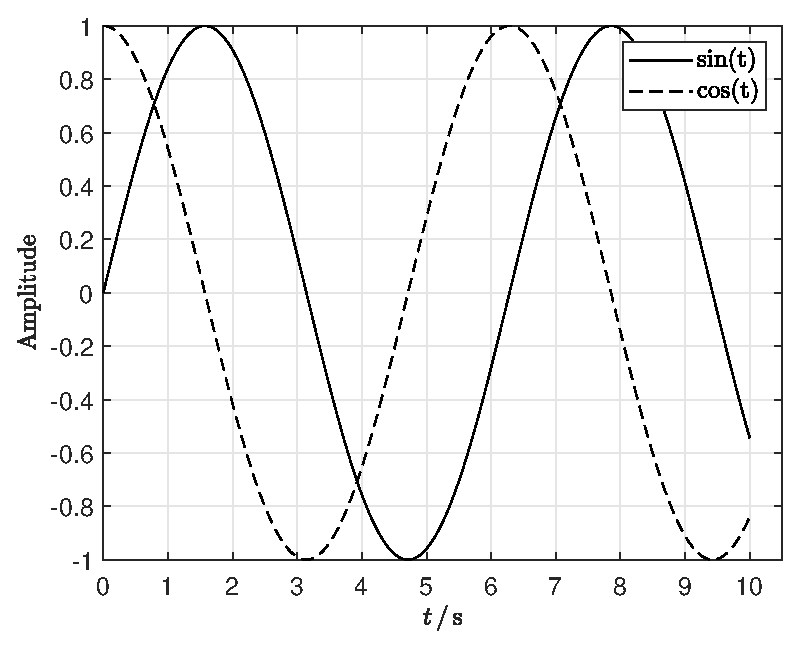
\includegraphics[width=0.6\textwidth]{img/Test_plot_1.eps}
	\caption[60\,\% der Textbreite]{Sinus- und Cosinus-Verlauf über die Zeit dargestellt.}
	\label{fig:test_plot_1}
\end{figure}

Hier ein Beispiel für Zahlen:
\begin{itemize}
	\item \num{1234,56}  % Zahl mit Dezimaltrennzeichen
	\item \SI{2}{\meter^{-1}} % Einheit m^-1 ohne Bruch
	\item \SI{1.23e4}{\newton\meter} % Exponenten mit Punkt als Produkt
	\item \SI{1000}{\kilo\ohm} % Tausender ohne Trennzeichen
\end{itemize}


Testen ob die Symbole und die Akronyms richtig funktionieren \gls{sym:C}, oder auch \gls{sym:L}.

A \gls{acr:pcb} is a fundamental component in the electronics industry and is commonly used to mechanically support and electrically connect various electronic components, including \glspl{acr:ic}. The complex impedance of an inductor is given by the formula
\begin{equation}
	Z_\mathrm{L}=\mathrm{i}\omega\gls{sym:L}
	\label{eqn:testgleichung}
\end{equation}
where $\gls{sym:L}$ is the inductance of the inductor.\par 
In \cref{fig:test_plot_1} ist ein Testplot dargestellt. und die Gleichung wird auch referenziert \cref{eqn:testgleichung}
    \chapter{Zusammenfassung und Ausblick}

\section{Zusammenfassung}

Fassen Sie die Arbeit zusammen indem Sie auf die wichtigsten Ergebnisse eingehen. Da Sie die Arbeit als bekannt voraussetzen k"onnen, m"ussen Sie nicht auf Details der Vorgehensweise eingehen.

\section{Reflexion und Ausblick}

Hier k"onnen Sie "uber die Erreichung der Ziele, ihren pers"onlichen Lerneffekt und die Wichtigkeit des Erreichten reflektieren. Die Formulierung eines Ausblicks auf weitere notwendige Arbeiten zeigt, dass Sie sich stark mit dem Inhalt identifizieren.

    \chapter{Introduction}
\label{chapter:introduction}
\section{Sample text}
\label{section:sample_text}
\lipsum[1]
\section{Another sample text}
\label{section:another_sample_text}
\lipsum[2]
\chapter{Theoretical background}
\label{chapter:theoretical_bg}
\section{Some facts}
\label{section:some_facts}
\lipsum[1]
\section{Some more facts}
\label{section:some_more_facts}
\lipsum[2]
\chapter{Tips and Tricks}
\label{chapter:tips_and_tricks}
\section{Cross-referencing and citing}
\label{section:cross_ref_and_citing}

\begin{itemize}
	\item \num{1234,56}  % Zahl mit Dezimaltrennzeichen
	\item \SI{2}{\meter^{-1}} % Einheit m^-1 ohne Bruch
	\item \SI{1.23e4}{\newton\meter} % Exponenten mit Punkt als Produkt
	\item \SI{1000}{\kilo\ohm} % Tausender ohne Trennzeichen
\end{itemize}
\section{Circuits and graphs}
\label{section:circuits_and_graphs}
\Cref{fig:demo_circuit} shows a simple linear and time-independent circuit, which is created with the package \texttt{circuitikz}. When using the \texttt{tikzexternalize} feature, the \texttt{circuitikz} environment must be substituted with \texttt{tikzpicture}. 
\begin{figure}[htbp]
	\centering
	\begin{tikzpicture}[scale=1,transform shape,european inductors,european resistors,
    american voltages]
    % grid definition
    % \draw[step=0.5,black!20,thin] (-4,-2.5) grid (4,2.5);
    % circuit definition
    \draw (0,0) coordinate (A) to [R,l=$R_\mathrm{1}$] ++ (-3,0) coordinate (B);
    \draw (B) to [vsource,l=$V_\mathrm{1}$] ++ (0,-2) -- ++ (3,0) coordinate (C);
    \draw (C) to [R,l=$R_\mathrm{L}$] (A);
    \draw (A) to [R,l_=$R_\mathrm{2}$,*-] ++ (3,0) coordinate (D);
    \draw (D) to [vsource,l=$V_\mathrm{2}$] ++ (0,-2) to [short,-*] (C);
\end{tikzpicture}
% EOF
	\caption{A simple circuit}
	\label{fig:demo_circuit}
\end{figure}

Waveforms captured by an oscilloscope are depicte \cite{deutsch}, im Anhang ist dann ein weiterer
Code verknüpft siehe dazu \ref{lst:test_code} und in \cref{fig:demo_circuit} und \ref{fig:demo_circuit} ist ein Schaltkreis mit tikz gezeichnet.

    \pagenumbering{Roman} % use uppercase roman numerals for page numbering
	\setcounter{page}{\value{romanpagecount}} % set page number to the stored value
    \stepcounter{page} % increment the page counter
    \bibliography{IEEEabrv,mybibfile} % point BibTEX at the .bib files
	\addcontentsline{toc}{chapter}{\bibname}
    \clearpage
	\listoffigures % generate a list of all the figures
	\addcontentsline{toc}{chapter}{\listfigurename}
    \clearpage
	\listoftables % generate a list of all the tables
	\addcontentsline{toc}{chapter}{\listtablename}
	\clearpage
    \printglossary[type=acronym, title={Abkürzungsverzeichnis}] % input files created by MakeIndex
	\printglossary[type=symbolslist,style=symbolsliststyle, title={Symbolverzeichnis}]
    \appendix
    \chapter[Erster Anhang]{"Uberschrift des ersten Anhangs}\label{app-A}

Text Text Text Text Text Text Text Text Text Text Text Text Text Text Text Text Text Text Text Text Text Text Text Text ...


\end{document}
%%%%%%%%%%%%%%%%%%%%%%%%%%%%%%%%%%%%%%%%%%%%%%%%%%%%%%%%%%%%%%%%%%%%%%%%%%%%%%%%%%%%%%